%=============================================================================
%=============================================================================

\chapter{Getting Started}
\label{ch-Getting-Started}

Before writing any code:

\begin{enumerate}

\item
{\bf Choose a conceptual interface (see Sections
\ref{sec-What-are-conceptual-interfaces} and
\ref{sec-Which-conceptual-interface}).}
Generally, the choice is fairly obvious.  A structured-grid interface
is clearly inappropriate for an unstructured-grid application.  It is
desirable to use a more specific interface if appropriate, e.g., the
linear-algebraic interface is usable from any type of grid but will
involve much more user work and prevent access to some
grid-type-specific preconditioners.

\item 
{\bf Choose your desired solver strategy.}  For the typical user, this
will mean a single Krylov method and a single preconditioner.

\item 
{\bf Look up matrix requirements for each solver and preconditioner.}
Each specific solver and preconditioner has requirements from the
input matrix.  This information is provided in several places: Chapter
\ref{ch-Solvers}, the \hypre{} Reference Manual, and
the \hypre{} header files.

\item 
{\bf Choose a matrix class that is compatible with your solvers and
preconditioners and your conceptual interface.}  Note that some of the
interfaces currently only support one matrix class choice.

\end{enumerate}
Once the previous decisions have been made, it is time to code your
application to call \hypre{}:
\begin{enumerate}

\item
{\bf Build any necessary auxiliary structures for your chosen
conceptual interface.} This includes, e.g., the grid and stencil
structures if you are using the structured-grid interface.

\item
{\bf Build the matrix, solution vector, and right-hand-side vector
through your chosen conceptual interface.}  Each conceptual interface
provides a series of calls for entering information about your problem
into \hypre{}.

\item
{\bf Build solvers and preconditioners and set solver parameters
(optional).}  Some parameters like convergence tolerance are the same
across solvers, while others are solver specific.

\item
{\bf Call the solve function for the solver.}

\item
{\bf Retrieve desired information from solver.} Depending on your
application, there may be different things you may want to do with the
solution vector.  Also, performance information such as number of
iterations is typically available, though it may differ from solver to
solver.

\end{enumerate}

%-----------------------------------------------------------------------------

\section{A Simple Example}
\label{sec-Simple-Example}

The following code serves as a simple example of the usage of \hypre{}.  In
this example, the structured-grid interface (discussed in Chapter
~\ref{ch-Struct}) is used to enter the problem into \hypre{}, and the
\code{PFMG} Multigrid solver is used to solve the system.  Since the
structured-grid interface currently only supports one underlying matrix class,
there are no choices to make here.  If we were using the semi-structured grid
interface instead, then we would have to choose between the \code{SStruct} and
\code{ParCSR} matrix classes, depending on the solver we want to use.

This example and all other examples in this manual are written in C,
but \hypre{} also supports Fortran.  See Section
\ref{sec-Fortran} for details.

\begin{display}
\begin{verbatim}

/*-----------------------------------------------------------
 * Set up the grid and stencil
 *-----------------------------------------------------------*/

HYPRE_StructGridCreate(MPI_COMM_WORLD, dim, &grid);
HYPRE_StructGridSetExtents(grid, ilower, iupper);
...
HYPRE_StructGridAssemble(grid);
	
HYPRE_StructStencilCreate(dim, stencil_size, &stencil);
HYPRE_StructStencilSetElement(stencil, 0, offset0);
...

/*-----------------------------------------------------------
 * Set up the matrix, right-hand side, and initial guess
 *-----------------------------------------------------------*/

HYPRE_StructMatrixCreate(MPI_COMM_WORLD, grid, stencil, &A);
HYPRE_StructMatrixInitialize(A);
HYPRE_StructMatrixSetBoxValues(A, ilower, iupper, nelts, elts, Avalues);
...
HYPRE_StructMatrixAssemble(A);

HYPRE_StructVectorCreate(MPI_COMM_WORLD, grid, &b);
HYPRE_StructVectorInitialize(b);
HYPRE_StructVectorSetBoxValues(b, ilower, iupper, bvalues);
...
HYPRE_StructVectorAssemble(b);

HYPRE_StructVectorCreate(MPI_COMM_WORLD, grid, &x);
HYPRE_StructVectorInitialize(x);
HYPRE_StructVectorSetBoxValues(x, ilower, iupper, xvalues);
...
HYPRE_StructVectorAssemble(x);

/*-----------------------------------------------------------
 * Set up the solver
 *-----------------------------------------------------------*/

HYPRE_StructPFMGCreate(MPI_COMM_WORLD, &solver);
HYPRE_StructPFMGSetMaxIter(solver, 50);     	 /* optional */
HYPRE_StructPFMGSetTol(solver, 1.0e-06);    	 /* optional */
HYPRE_StructPFMGSetup(solver, A, b, x);

/*-----------------------------------------------------------
 * Solve the linear system
 *-----------------------------------------------------------*/

HYPRE_StructPFMGSolve(solver, A, b, x);

/*-----------------------------------------------------------
 * Get solution info and free up memory
 *-----------------------------------------------------------*/

HYPRE_StructVectorGetBoxValues(x, ilower, iupper, xvalues);
...

HYPRE_StructPFMGDestroy(solver);
HYPRE_StructGridDestroy(grid);
HYPRE_StructStencilDestroy(stencil);
HYPRE_StructMatrixDestroy(A);
HYPRE_StructVectorDestroy(b);
HYPRE_StructVectorDestroy(x);

\end{verbatim}
\end{display}

%-----------------------------------------------------------------------------

\section{What are conceptual interfaces?}
\label{sec-What-are-conceptual-interfaces}

\begin{figure}
\centering
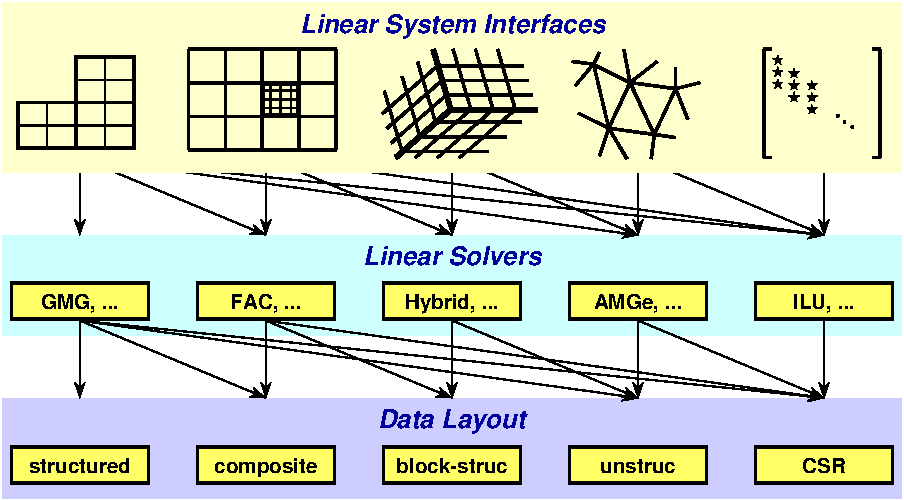
\includegraphics[width=5in]{fig_concep_iface}
\caption{%
Graphic illustrating the notion of conceptual interfaces.
All of these elements are not necessarily in \hypre{}.}
\label{fig-conceptual-interface}
\end{figure}

The top row of Figure~\ref{fig-conceptual-interface} illustrates a number of
conceptual interfaces.  Generally, the conceptual interfaces are denoted by
different types of computational grids, but other application features might
also be used, such as geometrical information.  These conceptual interfaces are
intended to represent the way that applications developers naturally think of
their linear problem, and provide natural interfaces for them to pass the data
that defines their linear system into \hypre{}.  Essentially, these conceptual
interfaces can be considered convenient utilities for helping a user build a
matrix data structure for \hypre{} solvers and preconditioners.  For example,
applications that use structured grids (such as in the left-most interface in
the Figure~\ref{fig-conceptual-interface}) typically view their linear problems
in terms of stencils and grids.  On the other hand, applications that use
unstructured grids and finite elements typically view their linear problems in
terms of elements and element stiffness matrices.  Finally, the right-most
interface is the standard linear-algebraic (matrix rows/columns) way of viewing
the linear problem.

The second row of Figure~\ref{fig-conceptual-interface} is a set of
linear solver algorithms.  Each linear solver group requires different
information from the user through the conceptual interfaces.  So, the
geometric multigrid algorithm (GMG) listed in the left-most box, for
example, can only be used with the left-most conceptual interface.  On
the other hand, the ILU algorithm in the right-most box may be used
with any conceptual interface.

The third row of Figure~\ref{fig-conceptual-interface} is a list of
data layouts or matrix/vector storage schemes.  The relationship
between linear solver and storage scheme is similar to that of
interface and linear solver.

%-----------------------------------------------------------------------------

\section{Which conceptual interface should I use?}
\label{sec-Which-conceptual-interface}

\hypre{} currently supports four conceptual interfaces:

\begin{itemize}

\item
{\bf Structured-Grid System Interface (\code{Struct}):} This interface is
appropriate for applications whose grids consist of unions of logically
rectangular grids with a fixed stencil pattern of nonzeros at each grid point.
This interface supports only a single unknown per grid point.  See Chapter
\ref{ch-Struct} for details.

\item
{\bf Semi-Structured-Grid System Interface (\code{SStruct}):} This
interface is appropriate for applications whose grids are mostly
structured, but with some unstructured features.  Examples include
block-structured grids, composite grids in structured adaptive mesh
refinement (AMR) applications, and overset grids.  This interface
supports multiple unknowns per cell.
See Chapter \ref{ch-SStruct} for details.

\item
{\bf Finite Element Interface (\code{FEI}):} This is appropriate for
users who form their linear systems from a finite element
discretization.  The interface mirrors typical finite element data
structures, including element stiffness matrices.  Though this
interface is provided in \hypre{}, its definition was determined
elsewhere (please email to Alan Williams william@sandia.gov for
more information).  See Chapter \ref{ch-FEI} for details.

\item
{\bf Linear-Algebraic System Interface (\code{IJ}):} This is the
traditional linear-algebraic interface.  It can be used as a last
resort by users for whom the other grid-based interfaces are not
appropriate.  It requires more work on the user's part, though still
less than building parallel sparse data structures.  General solvers
and preconditioners are available through this interface, but not
specialized solvers which need more information.  Our experience is
that users with legacy codes, in which they already have code for
building matrices in particular formats, find the IJ interface
relatively easy to use.
See Chapter \ref{ch-IJ} for details.

\end{itemize}

Generally, a user should choose the most specific interface that
matches their application, because this will allow them to use
specialized and more efficient solvers and preconditioners without
losing access to more general solvers.
